\documentclass[12pt]{article}
\usepackage{geometry}
\geometry{a4paper, margin=1in}
\usepackage{titlesec}
\usepackage{fancyhdr}
\usepackage{listings}
\usepackage{xcolor}
\usepackage{graphicx}
\usepackage{longtable}
\usepackage{caption}
\usepackage{hyperref}
\usepackage{graphicx}

\hypersetup{colorlinks=true, linkcolor=blue, urlcolor=blue}

\titleformat{\section}{\Large\bfseries}{\thesection}{1em}{}
\pagestyle{fancy}
\fancyhf{}
\rhead{Computer Network Lab}
\lhead{Dynamic NAT}
\rfoot{\thepage}

\begin{document}

\begin{titlepage}
    \centering
    \vspace*{2cm}
    
    {\Huge \bfseries Dynamic NAT Configuration in Cisco Packet Tracer\par}
    \vspace{2cm}
    
    {\Large \textbf{Computer Network Lab Report}\par}
    \vspace{1.5cm}
    
    {\large Submitted By: Your Name\par}
    \vspace{0.5cm}
    {\large Roll Number: 12345678\par}
    \vspace{0.5cm}
    {\large Department of Computer Science and Engineering\par}
    \vspace{0.5cm}
    {\large Your University Name\par}
    
    \vfill
    
    {\large Date: \today\par}
\end{titlepage}


\section*{Objective}
To implement and understand the working of \textbf{Dynamic NAT (Network Address Translation)} using Cisco Packet Tracer, allowing private IP addresses to access a public network by translating them dynamically to a public IP pool.

\section*{Tools Used}
\begin{itemize}
  \item Cisco Packet Tracer
  \item Routers (2x: Public Router \& NAT Router)
  \item Switches (1 or more)
  \item End Devices (PC, Server)
  \item Copper Cross-Over \& Serial DCE cables
\end{itemize}

\section*{Network Design Overview}
\begin{longtable}{|p{4cm}|p{4cm}|p{4cm}|}
\hline
\textbf{Device} & \textbf{Interface} & \textbf{IP Address / Role} \\
\hline
PC & NIC & 192.168.30.2 (Internal User Device) \\
\hline
Public Router & Fa0/0 & 192.168.30.1 (Gateway to NAT Router) \\
\hline
Public Router & S2/0 & 20.0.0.2 (Link to NAT Router) \\
\hline
NAT Router & S2/0 & 20.0.0.1 (NAT Inside) \\
\hline
NAT Router & Fa0/0 & 10.0.0.1 (NAT Outside) \\
\hline
Server & NIC & 10.0.0.100 (External Server) \\
\hline
\end{longtable}

\begin{figure}[h!]
\centering
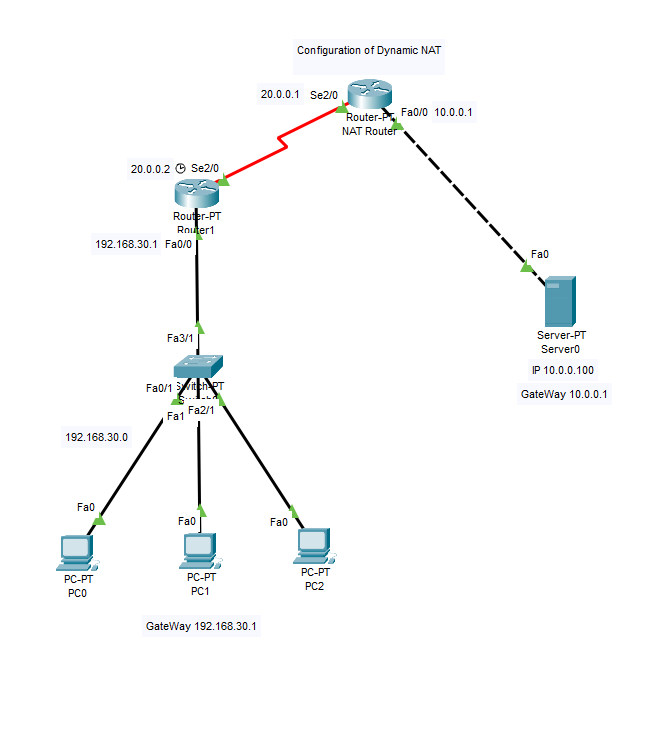
\includegraphics[width=1\textwidth]{topology.png}
\caption{Network Topology for Dynamic NAT Configuration}
\label{fig:topology}
\end{figure}


\section*{Step-by-Step Configuration}

\subsection{PC Configuration}
\begin{lstlisting}
IP Address: 192.168.30.2, 192.168.30.3 & 192.168.30.4
Subnet Mask: 255.255.255.0
Default Gateway: 192.168.30.1
\end{lstlisting}

\subsection{Public Router Configuration}
\begin{lstlisting}[language=bash]
enable
configure terminal

interface fa0/0
ip address 192.168.30.1 255.255.255.0
no shutdown
exit

interface s2/0
ip address 20.0.0.2 255.255.255.252
clock rate 64000
no shutdown
exit

ip route 0.0.0.0 0.0.0.0 20.0.0.1
\end{lstlisting}

\subsection{NAT Router Configuration}
\begin{lstlisting}[language=bash]
enable
configure terminal

interface s2/0
ip address 20.0.0.1 255.255.255.252
ip nat inside
no shutdown
exit

interface fa0/0
ip address 10.0.0.1 255.255.255.0
ip nat outside
no shutdown
exit

ip nat pool DYN_POOL 10.0.0.20 10.0.0.30 netmask 255.255.255.0
access-list 1 permit 192.168.30.0 0.0.0.255
ip nat inside source list 1 pool DYN_POOL overload

ip route 192.168.30.0 255.255.255.0 20.0.0.2
\end{lstlisting}

\subsection{Server Configuration}
\begin{lstlisting}
IP Address: 10.0.0.100
Subnet Mask: 255.255.255.0
Default Gateway: 10.0.0.1
\end{lstlisting}

\section*{Testing the Configuration}
\begin{itemize}
    \item From PC, run: \texttt{ping 10.0.0.100}
    \item On NAT Router, verify NAT translations:
\begin{lstlisting}[language=bash]
show ip nat translations
\end{lstlisting}
\end{itemize}

\noindent Output:
\begin{verbatim}
Pro  Inside Global     Inside Local     Outside Local     Outside Global
icmp 10.0.0.20:6       192.168.30.3:6     10.0.0.100:6       10.0.0.100:6
icmp 10.0.0.20:7       192.168.30.3:7     10.0.0.100:7       10.0.0.100:7
icmp 10.0.0.20:8       192.168.30.3:8     10.0.0.100:8       10.0.0.100:8
icmp 10.0.0.20:9       192.168.30.3:9     10.0.0.100:9       10.0.0.100:9
\end{verbatim}

\section*{Conclusion}
This lab successfully demonstrated how \textbf{Dynamic NAT} works in a network, allowing internal private IPs to dynamically be assigned public IPs from a pool when accessing an external network. The configuration ensures secure and controlled access between internal and external networks.

\end{document}
